\documentclass[12pt]{article}
\usepackage{a4wide, amsfonts, epsfig}
\newcommand\soln{\noindent\textit{Solution:} }


%skyline stuff
\font\upright=cmu10 scaled\magstep1
\setlength{\unitlength}{0.012500in}
\begingroup\makeatletter\ifx\SetFigFont\undefined
\def\x#1#2#3#4#5#6#7\relax{\def\x{#1#2#3#4#5#6}}%
\expandafter\x\fmtname xxxxxx\relax \def\y{splain}%
\ifx\x\y   % LaTeX or SliTeX?
\gdef\SetFigFont#1#2#3{%
  \ifnum #1<17\tiny\else \ifnum #1<20\small\else
  \ifnum #1<24\normalsize\else \ifnum #1<29\large\else
  \ifnum #1<34\Large\else \ifnum #1<41\LARGE\else
     \huge\fi\fi\fi\fi\fi\fi
  \csname #3\endcsname}%
\else
\gdef\SetFigFont#1#2#3{\begingroup
  \count@#1\relax \ifnum 25<\count@\count@25\fi
  \def\x{\endgroup\@setsize\SetFigFont{#2pt}}%
  \expandafter\x
    \csname \romannumeral\the\count@ pt\expandafter\endcsname
    \csname @\romannumeral\the\count@ pt\endcsname
  \csname #3\endcsname}%
\fi
\fi\endgroup

\begin{document}
\begin{center}
{\bf 2E2 Tutorial Sheet 16 Second Term, Solutions}\footnote{Conor
Houghton, {\tt houghton@maths.tcd.ie} and {\tt
http://www.maths.tcd.ie/\char126 houghton/ 2E2.html}}
\\[1cm]
 26 February 2006
\end{center}
{
\begin{enumerate}
\item (4) By linearizing around the critical points, draw the phase
plane portrait of
\begin{equation}
y''+y-y^3=0
\end{equation}
\vskip 1cm
\soln First, rewrite in first order form so let $y_1=y$ and define $y_2=y_1'$, now, from the equation $y_1''=y_2'=y_1^3-y_1$, putting these together gives:
\begin{eqnarray}
y_1'&=&y_2\cr
y_2'&=&y_1^3-y_1
\end{eqnarray}
The stationary points occur when $y_1'=y_2'=0$, hence $y_2=0$ and $y_1^3-y_1=0$, or, when $y_1=-1$ 0r $y_1=0$ or $y_1=1$. We will look at each of these stationary points in turn.
\vskip .5cm
Near $y_1=-1$ and $y_2=0$ we have $y_1=-1+\eta$ where $\eta$ is small. Hence
\begin{equation}
y_2'=(-1+\eta)^3-(-1+\eta)\approx-1+3\eta+1-\eta=2\eta
\end{equation}
and so, near this stationary point, the system is approximately 
\begin{eqnarray}
\eta'&=&y_2\cr
y_2'&\approx&2\eta
\end{eqnarray}
or
\begin{equation}
\left(\begin{array}{c}\eta\\y_2\end{array}\right)\approx\left(\begin{array}{cc}0&1\\2&0\end{array}\right)\left(\begin{array}{c}\eta\\y_2\end{array}\right)
\end{equation}
The matrix here has eigenvalues $\lambda_1=\sqrt{2}$ and
$\lambda_2=-\sqrt{2}$ with eigenvectors
\begin{equation}
{\bf x}_1=\left(\begin{array}{c}1\\ \sqrt{2}\end{array}\right)
\end{equation}
and
\begin{equation}
{\bf x}_2=\left(\begin{array}{c}1\\ -\sqrt{2}\end{array}\right)
\end{equation}
Hence, this stationary point is a saddle point and provided $\eta$ remains small, it is approximated by
\begin{equation}
\left(\begin{array}{c}\eta\\y_2\end{array}\right)\approx C_1{\bf x}_1e^{\sqrt{2}t}+C_2{\bf x}_2e^{-\sqrt{2}t}
\end{equation}
\vskip .5cm
Near $y_1=0$ and $y_2=0$ we assume both $y_1$ and $y_2$ are small and make the approximation 
\begin{equation}
y_2'=y_1^3-y_1\approx -y_1
\end{equation}
and so, near this stationary point, the system is approximately 
\begin{equation}
\left(\begin{array}{c}y_1\\y_2\end{array}\right)\approx\left(\begin{array}{cc}0&1\\-1&0\end{array}\right)\left(\begin{array}{c}y_1\\y_2\end{array}\right)
\end{equation}
This matrix has eigenvalues $\pm i$ and so this is a circle node.
\vskip .5cm
Near $y_1=1$ and $y_2=0$ we have $y_1=1+\eta$ where $\eta$ is small. Hence
\begin{equation}
y_2'=(1+\eta)^3-(1+\eta)\approx 2\eta
\end{equation}
and so, near this stationary point, the system is approximately 
\begin{equation}
\left(\begin{array}{c}\eta\\y_2\end{array}\right)\approx\left(\begin{array}{cc}0&1\\2&0\end{array}\right)\left(\begin{array}{c}\eta\\y_2\end{array}\right)
\end{equation}
and so this point is the same as the $y_1=-1$, $y_2=0$ stationary
point.
\begin{center}
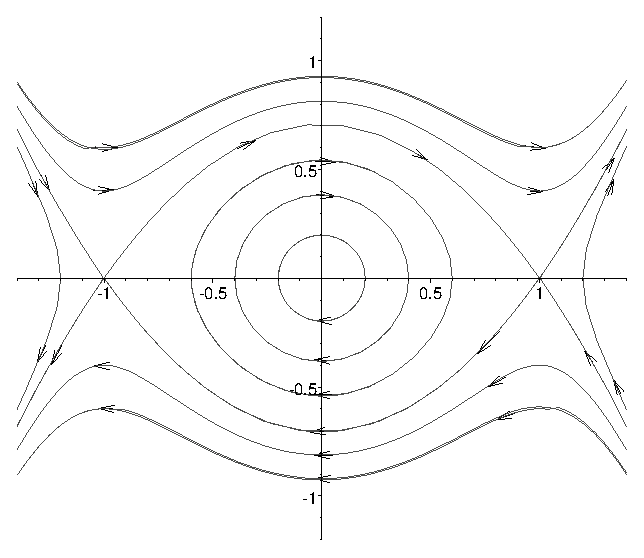
\epsfig{file=10Aug2003.eps, width=9cm}
\end{center}
\vskip 1cm
\item (4) By linearizing around the critical points, draw the phase
plane portrait of
\begin{equation}
y''=\cos{2y}
\end{equation}
\vskip .5cm
\soln  As before, rewrite as a first order system:
\begin{eqnarray}
y_1'&=&y_2\nonumber\\
y_2'&=&\cos{2y_1}
\end{eqnarray}
now, the critical points are located where $y_1'=y_2'=0$. This happens
when $y_2=0$ and $\cos{2y_1}=0$, that means $2y_1=n\pi/2$ where $n$ is
an odd integer, or $y_1=n\pi/4$ where again $n$ is an odd integer.
\vskip .5cm
Near $y_1=\pi/4$ write $y_1=\pi/4+\eta$ and use $\cos{2y_1}=\cos{2(\pi/4+\eta)}=-
\sin{2\eta}$ and this linearizes as $\sin{2\eta}\sim 2\eta$ so the system become
s
\begin{eqnarray}
\eta'&=&y_2\nonumber\\
y_2'&=&-2\eta.
\end{eqnarray}
This is a center. The matrix is
\begin{equation}
A=\left(\begin{array}{cc}0&1\\-2&0\end{array}\right)
\end{equation}
and so, by calculating the eigenvalues and eigenvectors, the general solution is
\begin{equation}
\left(\begin{array}{c}\eta\\y_2\end{array}\right)=c_1\left(\begin{array}{c}1\\ \sqrt{2}i\end{array}\right)e^{\sqrt{2}it}+c_2\left(\begin{array}{c}1\\ -\sqrt{2}i
\end{array}\right)e^{-\sqrt{2}it}
\end{equation} 
and by beginning at $\eta=r$ and $y_2=0$ we get
\begin{equation}
\left(\begin{array}{c}\eta\\y_2\end{array}\right)=r\left(\begin{array}{c}\cos{\sqrt{2}t}\\ -\sqrt{2}\sin{\sqrt{2}t}\end{array}\right)
\end{equation} 
so the saddle point is an ellipse with the vertical $\sqrt{2}$ times
as long as the horizontal.
\vskip .5cm
Near $y_1=3\pi/4$ write $y_1=3\pi/4+\eta$ and use $\cos{2y_1}=\cos{2(3\pi/4+\eta)}=\sin{2\eta}$ and this linearizes as $\sin{2\eta}\sim 2\eta$ so the system beco
mes
\begin{eqnarray}
\eta'&=&y_2\nonumber\\
y_2'&=&2\eta
\end{eqnarray}
This is a saddle-point with eigenvalues $\pm\sqrt{2}$ and eigenvectors
\begin{equation}
\left(\begin{array}{cc}1\\\pm\sqrt{2}\end{array}\right).
\end{equation}
This pattern repeats by periodicity, the phase portrait is\\
\\
\begin{center}
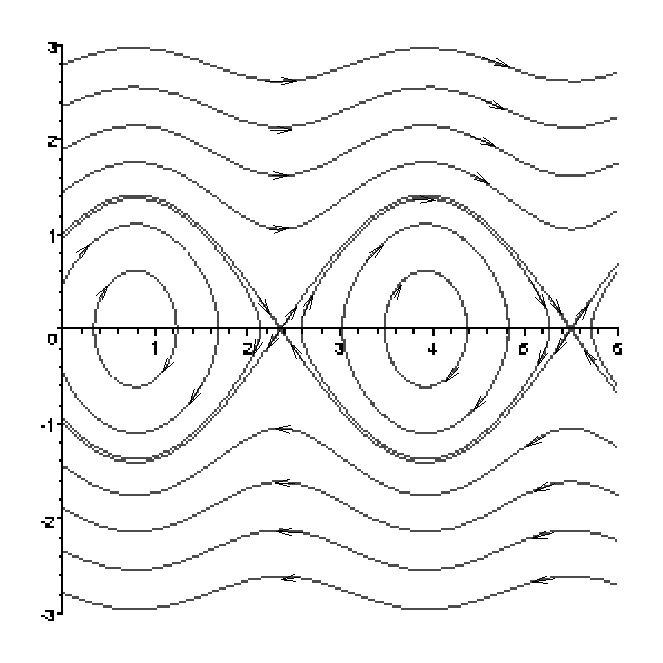
\epsfig{file=12Feb2001.eps, width=9cm}
\end{center}
\end{enumerate}
}
\end{document}



